\section{Parallélisation de NTMIX} \label{sec:part2}


Comme vu dans l'introduction, l'objectif est de pouvoir exécuter cette application sur un maillage de taille conséquente ($\approx 10^9$ points) ce qui est impossible de faire sur un unique processeur; en effet, pour chaque point d'un maillage, au moins 5 variables conservatives doivent être stockées (masse volumique, vitesses et l'énergie). Chacune de ces variables sont des nombres à virgule flottante en double précision (méthode utilisée pour représenter les nombres réels en informatique) occupant 8 octets. L'espace nécessaire pour stocker ces variables serait de $10^9 \times 5 \times 8 \approx 37.25$ Go, auquel il faudrait ajouter les $7.45$ Go par espèce chimique. Sachant qu'un des tests qui sera utilisé possédera 27 espèces, nous arrivons à un total de $37.25+27 \times 7.45\approx 238.42$ Go seulement pour stocker les variables nécessaires à la simulation auxquels il faudrait encore ajouter les tableaux de travail.

De plus, la charge de calcul serait colossale; les mesures de la version séquentielle présentées dans la section \ref{fig:vecto} montrent que pour un maillage d'environ 41 millions de points, le temps par point est de 4 $\mu$s. Dans le cas optimiste où ce temps n'augmenterait pas lorsqu'on augmente le nombre de points, un pas de temps pour $10^9$ points durerait $10^9\times4\times10^{-6}=4000$s ($\approx$ 1 heure 7 minutes). Une simulation de 10000 pas de temps durerait donc $4000\times10^4$ secondes $\approx$ 463 jours.


\subsection{Décomposition de domaine}
\paragraph{}Il est donc impératif de diviser la charge de travail ainsi que la mémoire utilisée par le programme afin d'arriver à des coûts en mémoire et CPU plus raisonnables. Pour cela, il est possible de partitionner le domaine de la simulation en plusieurs sous-domaines, plus petits, et de réaliser les calculs de chaque sous-domaine sur des processus différents, possédant chacun les données relatives à son sous-domaine. 

\paragraph{}MPI (\textit{Message Passing Interface}) décrit une librairie permettant de définir des topologies virtuelles et les transferts de données entre les nœuds d'une telle topologie et permettra donc de diviser le domaine selon une grille cartésienne de processus. Chaque case d'une topologie calculera une petite partie de la solution globale mais pourra le faire en parallèle des autres. La figure \ref{fig:globaldom} représente un domaine en 2D avec en bleu ses bordures physiques. La figure \ref{fig:partdom} montre un partitionnement de ce domaine en 4 sous-domaines, chacun possédant de nouvelles bordures.


\begin{figure}[!ht]
  \centering
  \begin{subfigure}[b]{0.5\textwidth}
    \centering
    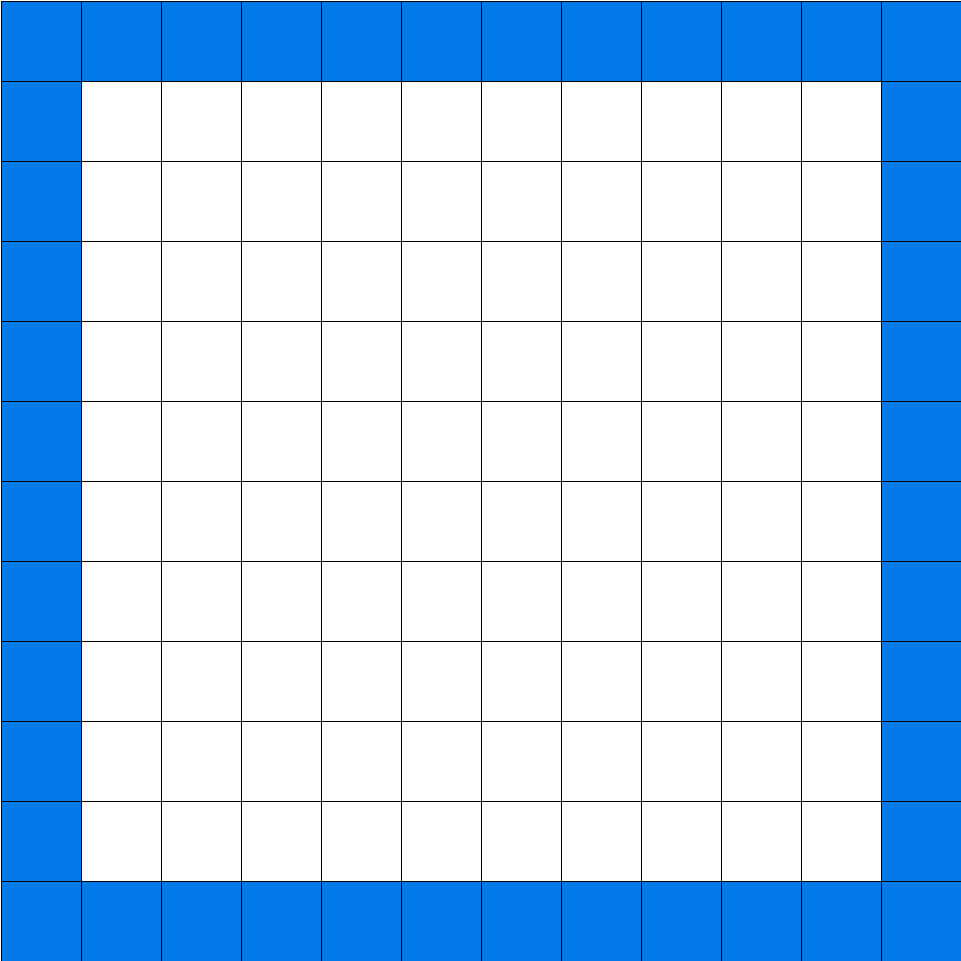
\includegraphics[scale=0.15]{figures/globaldomain.png}
  \caption{\label{fig:globaldom}Domaine complet}
  \end{subfigure}%
  ~
  \begin{subfigure}[b]{0.5\textwidth}
    \centering
    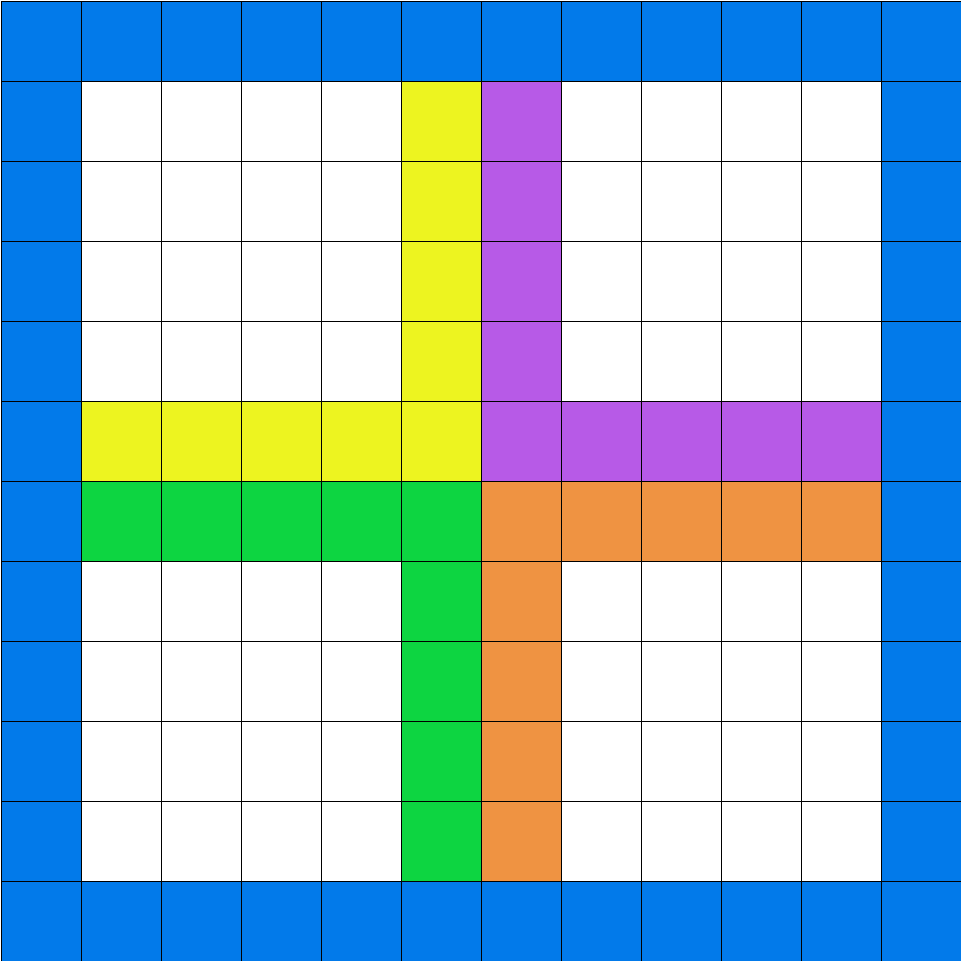
\includegraphics[scale=0.15]{figures/partitionnedomain.png}
  \caption{\label{fig:partdom}Domaine partitionné}
  \end{subfigure}
  \caption{\label{fig:dom}Partitionnement du domaine}
\end{figure}


\paragraph{}Cependant, pour résoudre les équations aux dérivées partielles (\textit{PDEs: Partial Differential Equations}) lorsque le domaine est partitionné, il faut utiliser des méthodes de décomposition de domaine. Ces sont des méthodes numériques permettant de résoudre des problèmes d'algèbre linéaire sur des machines parallèles, notamment dans le cadre des simulations scientifiques, en modifiant le traitement réalisé sur les bordures artificielles (bordures induites par la décomposition).\cite{dolean+jolivet+nataf}


\subsubsection{Approche numérique}\label{sec:numerical_dom_decompo}

\paragraph{}Chaque processus ne peut donc pas travailler de manière totalement indépendante. Dans NTMIX, une méthode compacte est utilisée pour calculer les gradients des différents champs \cite{Hirsch:1988:NCI:63653}. Pour les points ne se trouvant pas sur les bordures du domaine, la dérivée au point $u$ sur la direction $x$ est calculée grâce au schéma:

\begin{equation}\label{eq:pade}
3\left( \frac{\partial u}{\partial x}\right) _{i-1} + 9\left( \frac{\partial u}{\partial x}\right) _{i} + 3\left( \frac{\partial u}{\partial x}\right) _{i+1} = \frac{1}{h}\left(  \frac{1}{4} \left( u_{i+2}-u_{i-2} \right) + 7 \left( u_{i+1} - u_{i-1} \right) \right) 
\end{equation}


$\left( \frac{\partial u}{\partial x}\right) _{i}$ est donc dépendante des 2 situés en $(i-1)$ et $(i-2)$ et des 2 points $(i+1)$ et $(i+2)$ mais aussi des dérivées en $(i-1)$ et $(i+1)$. Une telle méthode implique donc que la dérivée en un point est dépendante des valeurs de tous les autres points du champ. 


 Comme on peut le voir sur la figure \ref{fig:dependencies}, après le partitionnement du domaine, les points se trouvant sur les bordures internes (bordures entre processus) manquent d'information pour réaliser les calculs, pouvant entraîner une perte de précision des résultats de la simulation. Pour résoudre ce problème, il est possible de créer des zones de recouvrement entre les différents sous-domaines, permettant ainsi d'avoir accès aux points nécessaires aux calculs des dérivées. Ces zones sont représentées en gris sur la figure \ref{fig:depdomover} (ici les zones de recouvrement sont représentées par une seule case pour la clarté du schéma mais la taille de ces zones dépend de la méthode numérique utilisée). L'ensemble des schémas sont également en 2D pour faciliter la lecture.



\begin{figure}[!ht]
  \centering
  \begin{subfigure}[b]{0.5\textwidth}
    \centering
    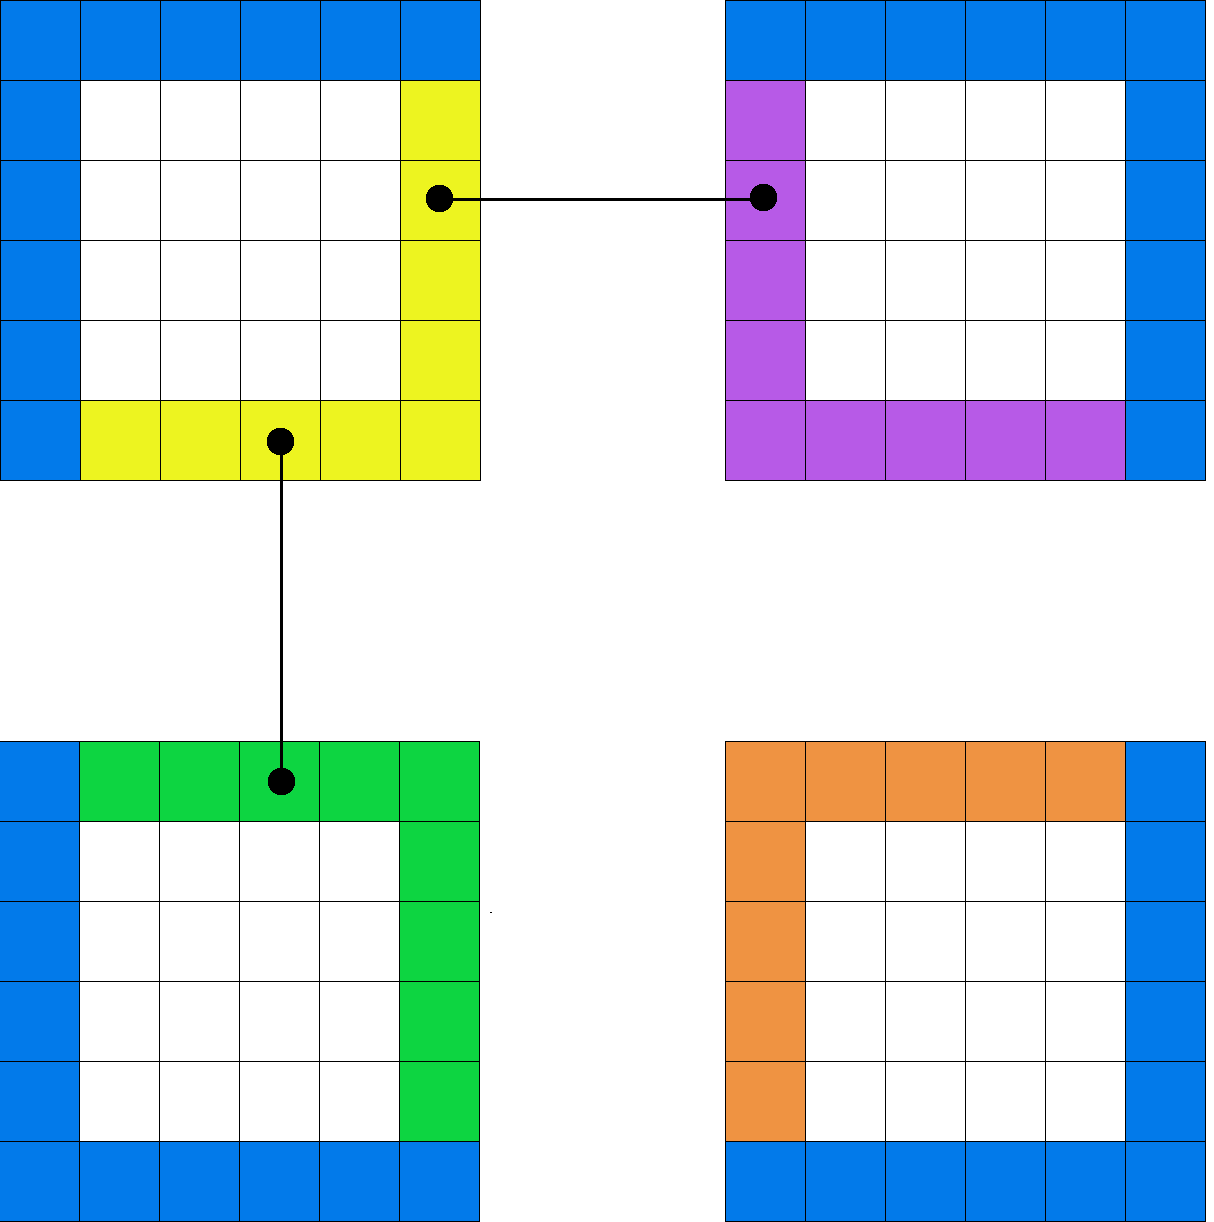
\includegraphics[scale=0.15]{figures/depdomain.png}
  \caption{\label{fig:dependencies} }
  \end{subfigure}%
  ~
  \begin{subfigure}[b]{0.5\textwidth}
    \centering
    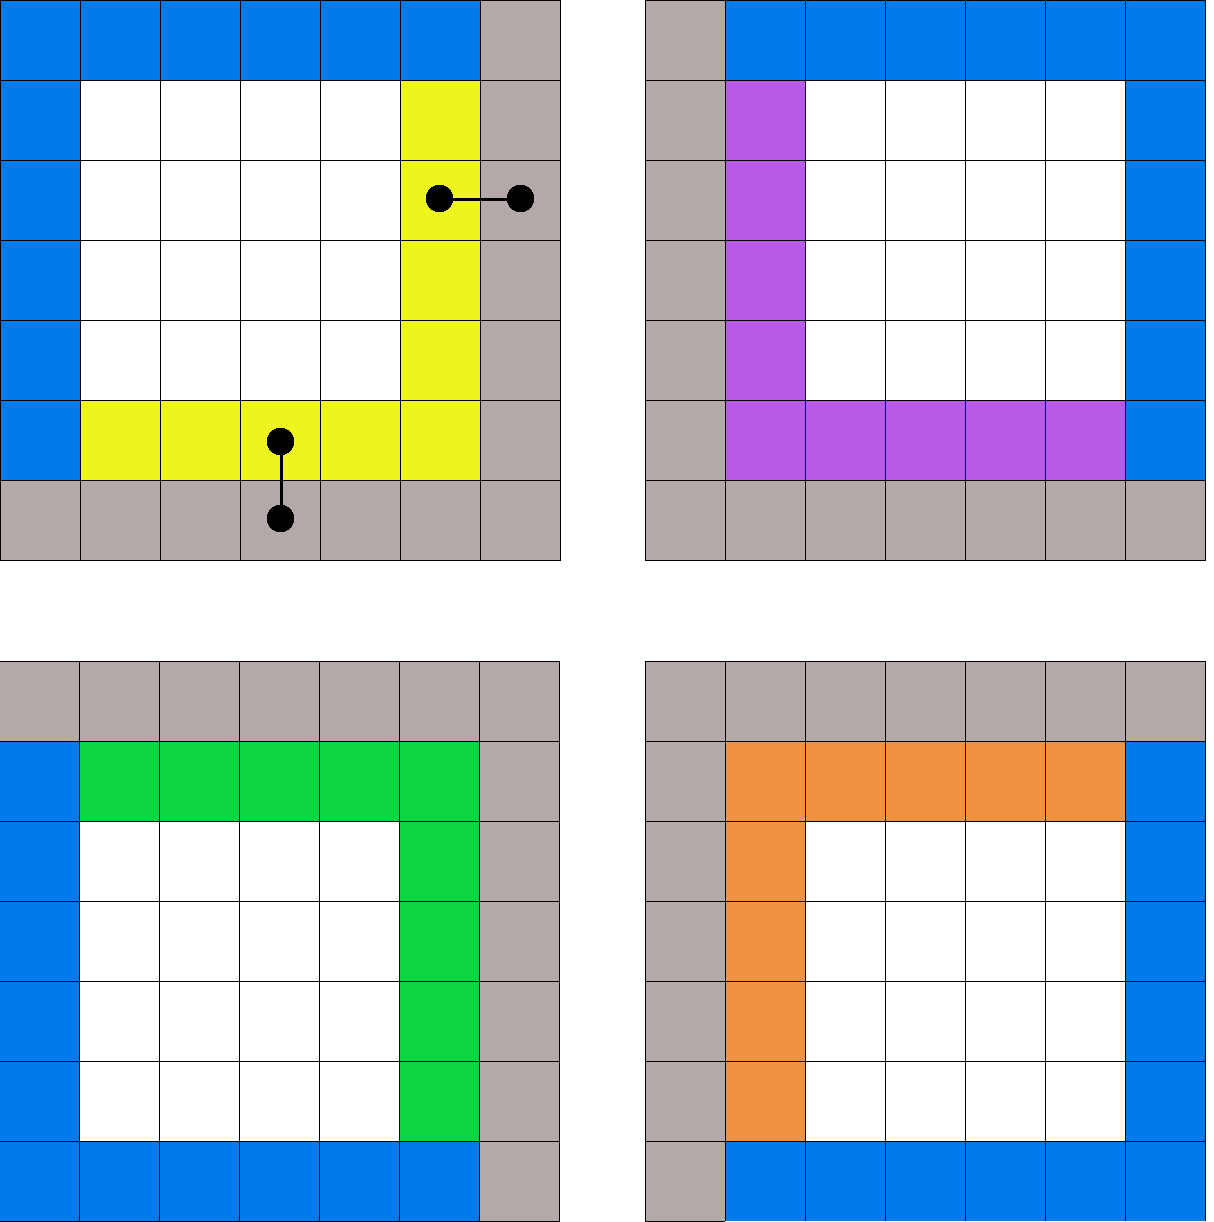
\includegraphics[scale=0.15]{figures/depdomain-overlap.png}
  \caption{\label{fig:depdomover} }	
  \end{subfigure}
  \caption{\label{fig:domdep}Recouvrement entre les sous-domaines}
\end{figure}




\paragraph{}La mise en œuvre efficace de l'approche numérique présentée ci-dessus sur les plates-formes parallèles a fait l'objet d'études \cite{Stoessel:1994:DNS:199617.199626,Hirsch:1988:NCI:63653} et la résolution par décomposition de domaine semble être la plus efficace. Le but est de résoudre localement le problème global. Nous nous intéressons ici aux 2 approches présentées dans l'étude \cite{Baum98dnsof}:

\paragraph{Méthode Schwarz}: elle consiste à résoudre chaque sous-système avec des conditions limites de type Dirichlet, permettant de spécifier les valeurs que la solution doit prendre sur les bordures d'un domaine. Pour cela, l'expression (\ref{eq:pade}) est modifiée sur les frontières par:

\begin{equation}\label{eq:dirichlet}
3\left( \frac{\partial u}{\partial x}\right) _{i-1} + 9\left( \frac{\partial u}{\partial x}\right) _{i}  = \frac{1}{h}\left(  \frac{1}{4} \left( u_{i+2}-u_{i-2} \right) + 7 \left( u_{i+1} - u_{i-1} \right) \right) - 3 \delta u_{i+1}
\end{equation}

Le terme $3 \delta u_{i+1}$ est une approximation de la dérivée sur la frontière calculée par le domaine adjacent. Cette méthode nécessite donc un couplage fort entre les sous-domaines adjacents.

\paragraph{Problème local modifié}: cette seconde méthode permet de réduire l'importance du couplage de la méthode précédente. Aux frontières des sous-domaines, le schéma utilisé pour les bordures physiques est appliqué \cite{Stoessel:1994:DNS:199617.199626}:

  \begin{subequations}
    \begin{align}
      2 \left( \frac{\partial u}{\partial x}\right) _{1} + 4 \left( \frac{\partial u}{\partial x}\right) _{2} &= \frac{1}{h}\left( u_3 + 4u_2 - 5u_1 \right)\label{eq:schem1}
      \\
~
      4\left( \frac{\partial u}{\partial x}\right) _{n_x-1} + 2\left( \frac{\partial u}{\partial x}\right) _{n_x}  &= \frac{1}{h} \left( u_{n_x-2} + 4 u_{n_x-1} - 5 u_{n_x} \right)\label{eq:schemnx}
    \\
~
    \left( \frac{\partial u}{\partial x}\right) _{i-1} + 4 \left( \frac{\partial u}{\partial x}\right) _{i}  +  \left( \frac{\partial u}{\partial x}\right) _{i-1} &= \frac{1}{h}\left( \frac{1}{3} \left( u_{i+1} - u_{i-1} \right) \right)\label{eq:schem-2nx-1}
    \end{align}
  \end{subequations}

%$$\left( \frac{\partial u}{\partial x}\right) _{1} + 4 \left( \frac{\partial u}{\partial x}\right) _{2}  +  \left( \frac{\partial u}{\partial x}\right) _{3} = \frac{1}{h}\left( \frac{1}{3} \left( u_3 - u_1 \right) \right)$$
%$$\left( \frac{\partial u}{\partial x}\right) _{n_x-2} + 4 \left( \frac{\partial u}{\partial x}\right) _{n_x-1}  +  \left( \frac{\partial u}{\partial x}\right) _{n_x} = \frac{1}{h}\left( \frac{1}{3} \left( u_{n_x} - u_{n_x-2} \right) \right)$$


Les schémas (\ref{eq:schem1}) et (\ref{eq:schemnx}) sont appliqués pour les points $1$ et $n_x$; le schéma (\ref{eq:schem-2nx-1}) pour les points $i=2 \text{ et } i=n_x-1$. Ce sont des schémas décentrés qui réduisent donc la précision de la solution mais qui permettent de calculer un pas complet de l'intégration de Runge-Kutta (sec. \ref{sec:comms}), sans aucun couplage entre les sous-domaines. Du fait de leur précision moindre, il est cependant nécessaire d'utiliser des régions de recouvrement plus grandes qu'avec la méthode précédente.
%\end{itemize}



\subsubsection{Implémentation}
Au niveau de l'implémentation avec \textit{MPI} de ces méthodes, la première implique des communications pendant chaque calcul de dérivée, nombreux dans le code ($>100$ par pas de temps). La seconde méthode a l'avantage de grandement réduire le nombre de communications ($3$ par pas de temps) mais elles seront plus volumineuses; en effet pour la première méthode, seule une variable conservative sera communiquée à la fois mais pour la seconde méthode, l'ensemble des variables conservatives seront transmises entre les processus adjacents. Lors de l'utilisation de \textit{MPI}, il est d'usage de réduire au maximum les communications, qui entraînent des synchronisations et augmentent les temps d'attente entre les processus; c'est pour cette raison que la seconde méthode est choisie.


%Pour clarifier la suite du rapport, il est nécessaire de définir les termes se rapportant aux différentes bordures:
%
%\begin{itemize}
%\item bordures physiques: ce sont les bordures \textbf{globales} du domaine de calcul; celles représentées en couleur sur la figure \ref{fig:globaldom}
%\item bordures internes: ce sont les bordures des différents sous-domaines induites par le partitionnement du domaine; celles en couleur sur la figure \ref{fig:partdom}. Elle ne contiennent pas les bordures physiques.
%\item bordures de recouvrement: ce sont les bordures des sous-domaines après avoir ajouté les zones de recouvrement; elles sont représentées en gris sur la figure \ref{fig:depdomover}
%\end{itemize}

\paragraph{Calcul des gradients}
Maintenant que le domaine est décomposé, un sous-domaine peut posséder des bordures physiques et des bordures internes. Pour les différencier, le calcul des dérivées a été éclaté en briques élémentaires. Le schéma de la figure \ref{fig:dfdx_decompo} montre l'idée générale pour ce découpage. Le point d'entrée correspond à l'appel de la fonction \textit{dfdx} permettant de réaliser la dérivation d'une variable d'un sous-domaine selon l'axe $x$. Les fonctions \textit{dfdx\_$\alpha$\_lower} et \textit{dfdx\_$\alpha$\_upper} correspondent aux schémas utilisés pour la condition limite $\alpha$, respectivement sur les points $[1,2]$ et $[n_x-1,n_x]$. Les fonctions \textit{dfdx\_nrb\_lower} et \textit{dfdx\_nrb\_upper} correspondent aux schémas décentrés présentés en \ref{sec:numerical_dom_decompo} et utilisés sur les bordures internes. $pos_x$ correspond à la position du sous-domaine selon l'axe $x$ et $nproc_x$ au nombre de sous-domaines sur l'axe $x$; $pos_x=1$ et $pos_x=nproc_x$ indiquent que le sous-domaine se trouve respectivement sur les bordures physiques basses et hautes du domaine dans la direction $x$.


%Dans NTMIX, il existe 3 type de conditions limites (périodique, symétrique et double-symétrique). Pour ces 3 types de conditions, le schéma (\ref{eq:pade}) est appliqué sur les points $[3,n_x-2]$, indépendamment des conditions limites. Pour les points $[1,2]$ et $[n_x-1,n_x]$, le calcul des dérivées dépend de ces conditions limites. Cependant, pour chacune des conditions limites, une fonction différente réalise la dérivation sur l'ensemble $[1,n_x]$. Maintenant que le domaine est décomposé, il a fallu modifier cette façon de procéder car un sous-domaine ne possède plus forcement l'ensemble des bordures physiques et il est nécessaire d'appliquer les bons schémas de dérivation aux bordures internes. Pour cela, le calcul des dérivée a été éclatée en briques élémentaires. Le schéma \ref{fig:dfdx_decompo} montre l'idée générale derrière ce découpage. Le point d'entrée correspond à l'appel de la fonction \textit{dfdx} permettant de réaliser la dérivation d'une variable d'un sous-domaine selon l'axe $x$. Les fonctions \textit{dfdx\_$\alpha$\_lower} et \textit{dfdx\_$\alpha$\_upper} correspondent aux schémas utilisés par la condition limite $\alpha$, respectivement sur les points $[1,2]$ et $[n_x-1,n_x]$. Les fonctions \textit{dfdx\_nrb\_lower} et \textit{dfdx\_nrb\_upper} correspondent aux schémas des bordures non réfléchissantes (\textit{NRB: Non-Reflecting Boundaries}) présentés en \ref{sec:numerical_dom_decompo} et utilisés sur les bordures internes. $pos_x$ correspond à la position du sous-domaine selon l'axe $x$ et $nproc_x$ au nombre de sous-domaines sur l'axe $x$; $pos_x=1$ et $pos_x=nproc_x$ indiquent que le sous-domaine se trouve sur les bordures physiques du domaine. 

\begin{figure}[!ht]
  \centering
  %\includegraphics[scale=0.4]{figures/dfdx_decompo.pdf}
  \caption{\label{fig:dfdx_decompo} Calcul de gradient dans le cas d'un domaine décomposé}
\end{figure}


\paragraph{Recouvrement de domaines}\label{sec:overlapping}
Il existe 2 types de recouvrement possible dans NTMIX qui dépendent du type de conditions utilisées pour les bordures physiques:
\begin{itemize}
\item conditions périodiques: ce cas, utilisé pour éliminer les problèmes décrits en section \ref{sec:nsbc}, ne possède, par définition, pas de bordures physique et par conséquent, le recouvrement doit se produire entre tous les sous-domaines et dans toutes les directions. Chaque processus possédera 2 régions de recouvrement sur toutes les directions comme illustré sur la figure \ref{fig:per_overlap} (les cases grisées représentent le recouvrement).
\item conditions non-périodiques: dans ces cas, les propriétés physiques des bordures sont traitées, et les processus se trouvant en bord de domaine global selon une direction ne possèdent qu'une seule région de recouvrement selon cette direction (fig. \ref{fig:aper_overlap}). 
\end{itemize}

\begin{figure}[!ht]
  \centering
  \begin{subfigure}[b]{0.5\textwidth}
    \centering
    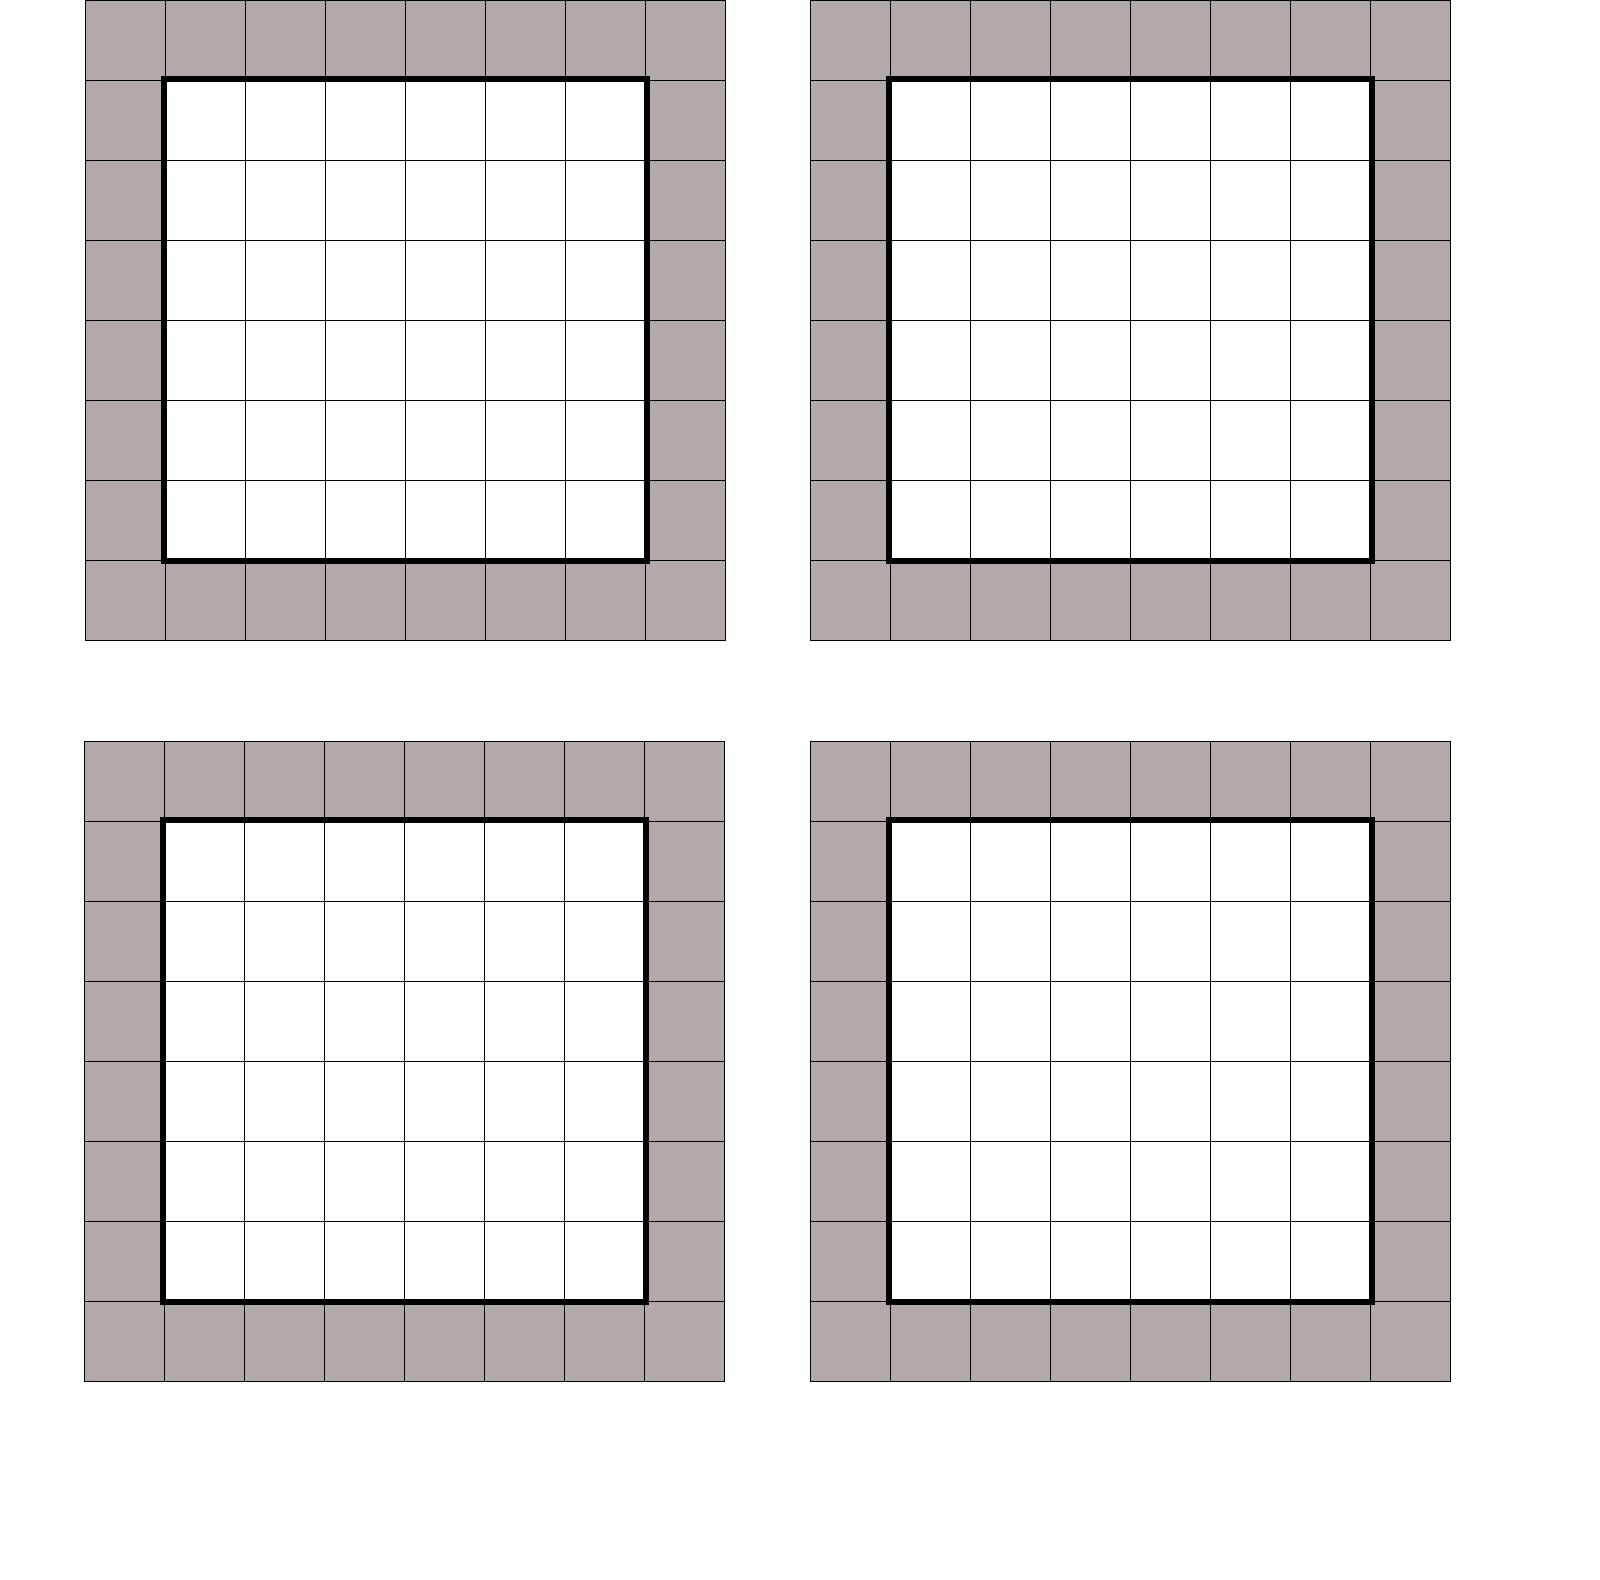
\includegraphics[scale=0.12]{figures/domain_per.png}
    \caption{\label{fig:per_overlap}Recouvrement périodique}
  \end{subfigure}%
  ~
  \begin{subfigure}[b]{0.5\textwidth}
    \centering
    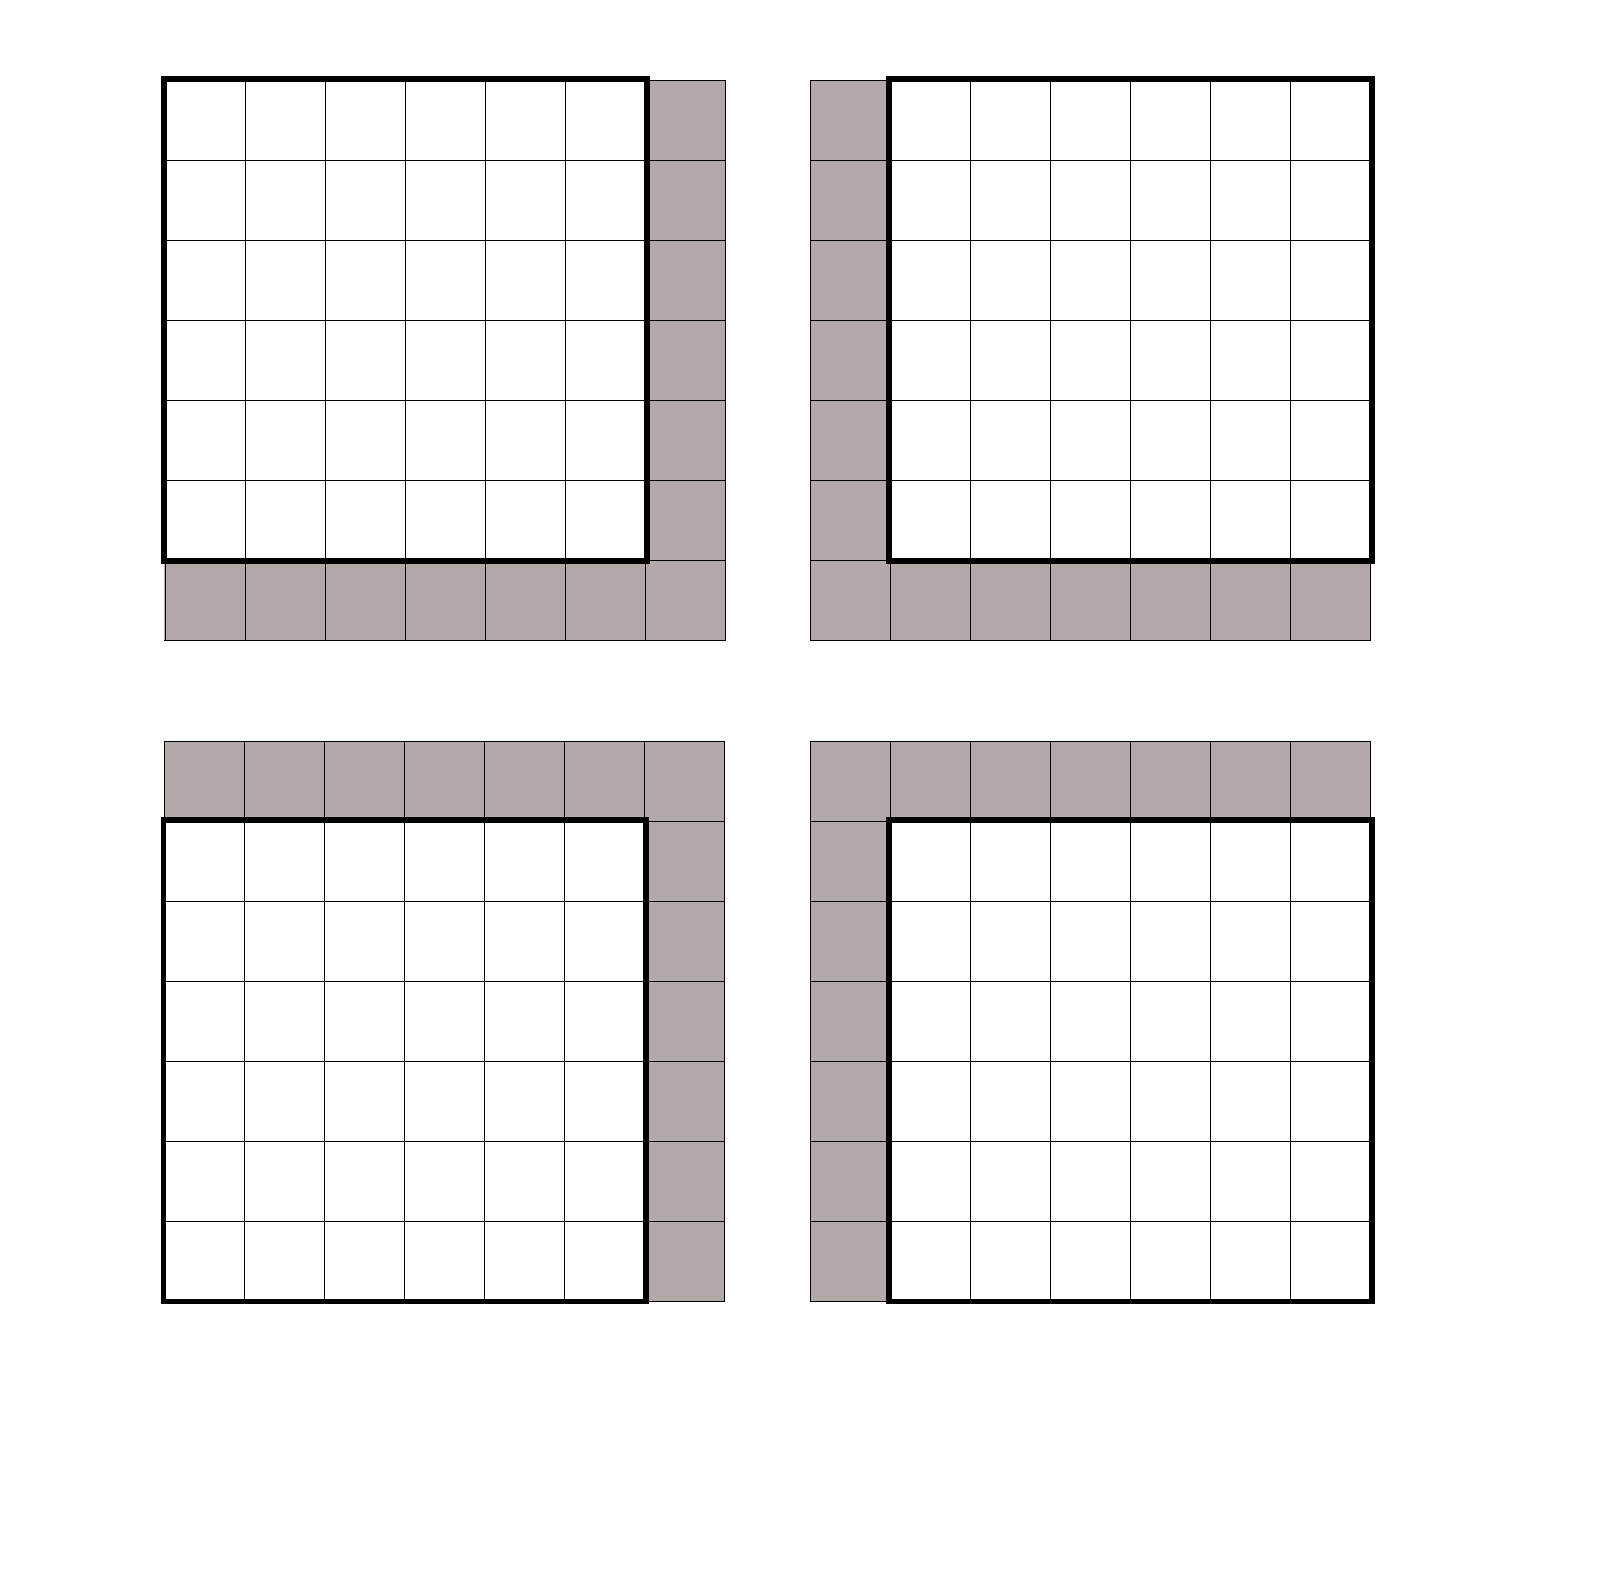
\includegraphics[scale=0.12]{figures/domain_aper.png}
    \caption{\label{fig:aper_overlap}Recouvrement apériodique}
  \end{subfigure}
  \caption{\label{fig:overlap_type}Types de recouvrement}
\end{figure}

\subsubsection{Traitement des bordures internes}
Sur la figure \ref{fig:depdomover}, on peut voir que lors du partitionnement du domaine, des bordures internes apparaissent. Ces bordures ne sont donc pas des bordures physiques et ne doivent, par conséquent, pas recevoir les traitements spécifiques à celles-ci.

Initialement, ce traitement était réalisé sur les 2 bords physiques d'une direction en même temps.
%Pendant chaque appel à la fonction RHS, les corrections présentées dans la section \ref{sec:nsbc} sont appliquées sur les bordures afin de réduire les instabilités numériques. Ces corrections sont réalisées par un noyau de calcul qui traite les 2 plans bordure sur chaque direction. Or, il est maintenant possible qu'un sous-domaine possède un seul ou aucun de ces plans. 
J'ai donc modifié ce code afin qu'il ne traite plus qu'un seul bord à la fois, et uniquement lorsque qu'un processus possède une bordure physique. 

%Des corrections sont également appliquées par rapport à la nature physique des bordures. En effet, différents comportements de frontière sont implémentés dans NTMIX. Ces corrections sont réalisées après chaque appel à RHS, dans la fonction \textit{impose\_boundary\_conditions} (algo \ref{algo:time_step}). Contrairement aux cas des \textit{NSCBC}, ces corrections s'effectuaient déjà sur un unique plan, mais maintenant, seul les sous-domaines avec des bordures physiques les appliqueront.


\subsection{Communications}\label{sec:comms}

\subsubsection{Calcul du pas de temps}
Dans la version séquentielle de NTMIX, un pas de temps maximum, permettant de garantir la stabilité de la simulation, est calculé sur l'ensemble du domaine.
Dans la version parallèle, chaque sous-domaine calcule son pas de temps maximal et une opération de réduction est utilisée pour trouver le maximum global. Elle permet de trouver le pas de temps maximal entre tous les sous-domaines et de le distribuer sur tous les processus.

\subsubsection{Transfert des points de recouvrement}

La discrétisation temporelle est réalisée avec une méthode de Runge-Kutta. C'est une méthode itérative; une première estimation de la solution est utilisée pour calculer une seconde estimation plus précise, et ainsi de suite \cite{Hirsch:1988:NCI:63653}. Dans NTMIX, 3 itérations sont réalisées à chaque pas de temps.
Comme vu dans la section précédente, la méthode de décomposition de domaine permet de calculer une itération complète. Il est donc nécessaire que les transferts des zones de recouvrement se fassent avant chaque appel à ces itérations afin que le calcul de l'intégration puisse se faire. Une fonction \textit{update} réalisera les communications et sera appelée avant chaque itération (algo \ref{algo:time_step}).


\begin{algorithm}
  \caption{time\_step}
  \label{algo:time_step}
  \begin{algorithmic}
     \STATE {Call Update}
     \STATE {Call RHS(1)} 
     \STATE {Call impose\_boundary\_conditions}
     \STATE {Call Update}	
     \STATE {Call RHS(2)} 
     \STATE {Call impose\_boundary\_conditions}
     \STATE {Call Update}
     \STATE {Call RHS(3)} 
     \STATE {Call impose\_boundary\_conditions}
  \end{algorithmic}
\end{algorithm}



\paragraph{}Dans cette fonction, chaque processus doit envoyer des informations sur ses bordures à tous ses voisins dans la topologie virtuelle. MPI fournit une fonction permettant de réaliser ce type de communication; MPI\_Neighbor\_alltoallv \cite{mpi-3.0}. Pour l'utiliser, il faut préparer un buffer qui contiendra les données à envoyer à chacun de ses voisins. La fonction gère automatiquement la répartition des buffers à envoyer aux voisins selon leur disposition sur la topologie. Après l'appel à cette fonction, le buffer de réception contient les données de tous les voisins autour d'un processus. Il ne reste plus qu'à stocker les variables reçues à leur place. 

\begin{figure}[!ht]
  \centering
  \begin{subfigure}[b]{0.5\textwidth}
    \centering
    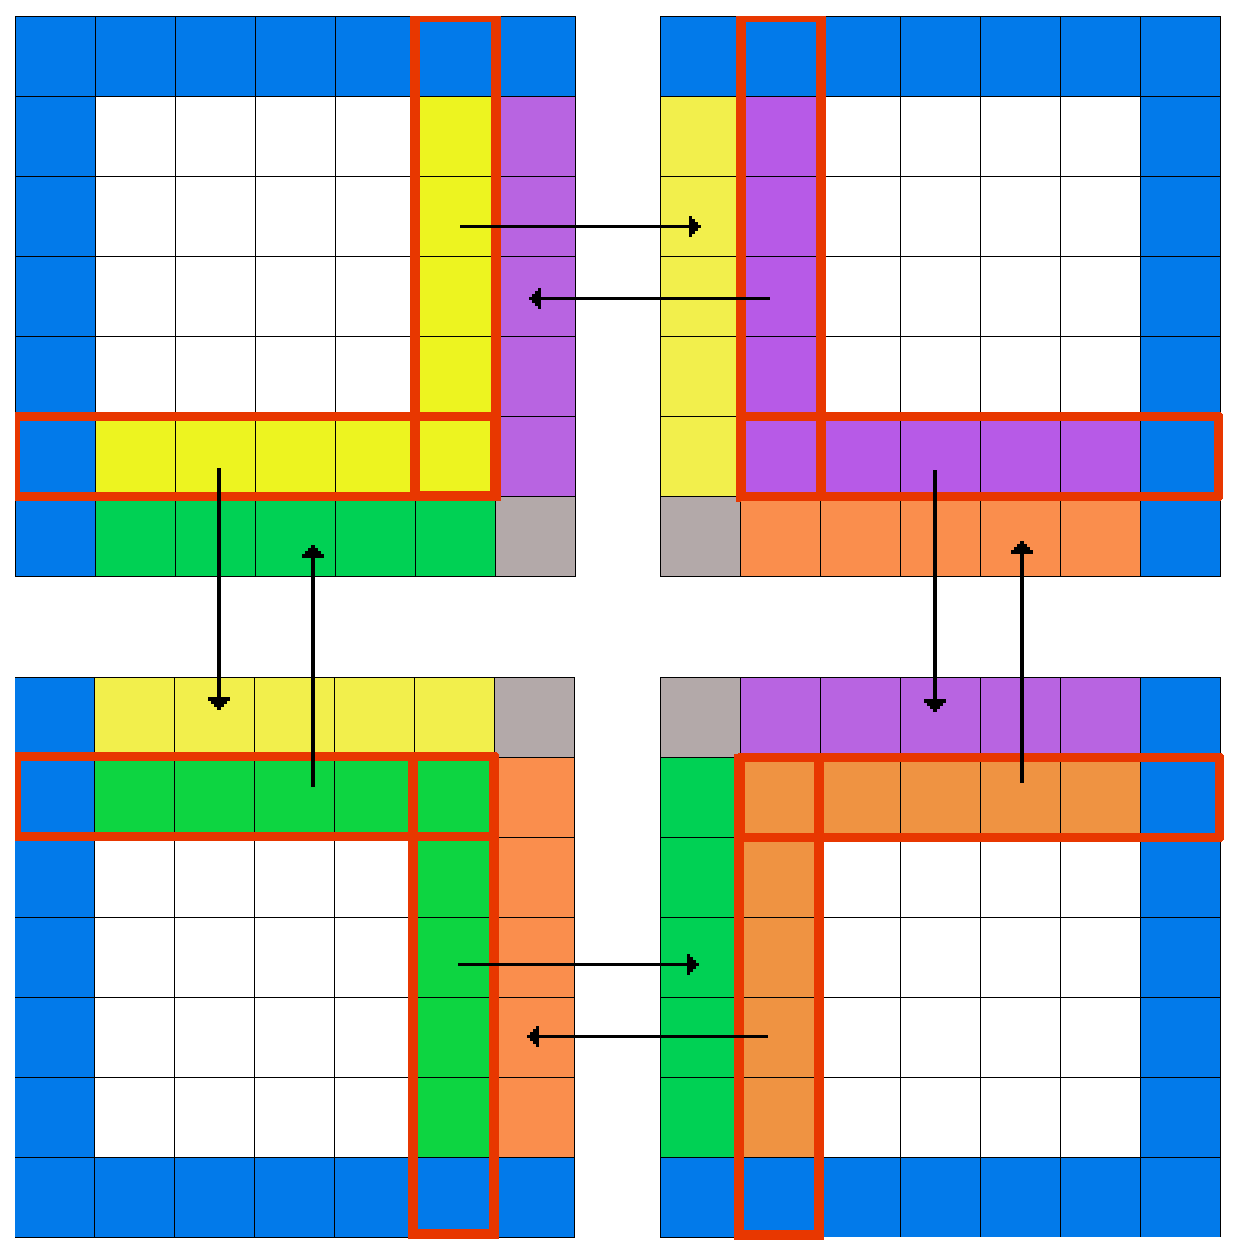
\includegraphics[scale=0.12]{figures/neigh1.png}
    \caption{\label{fig:comm_neigh}Echanges des zones de recouvrement}
  \end{subfigure}%
  ~
  \begin{subfigure}[b]{0.5\textwidth}
    \centering
    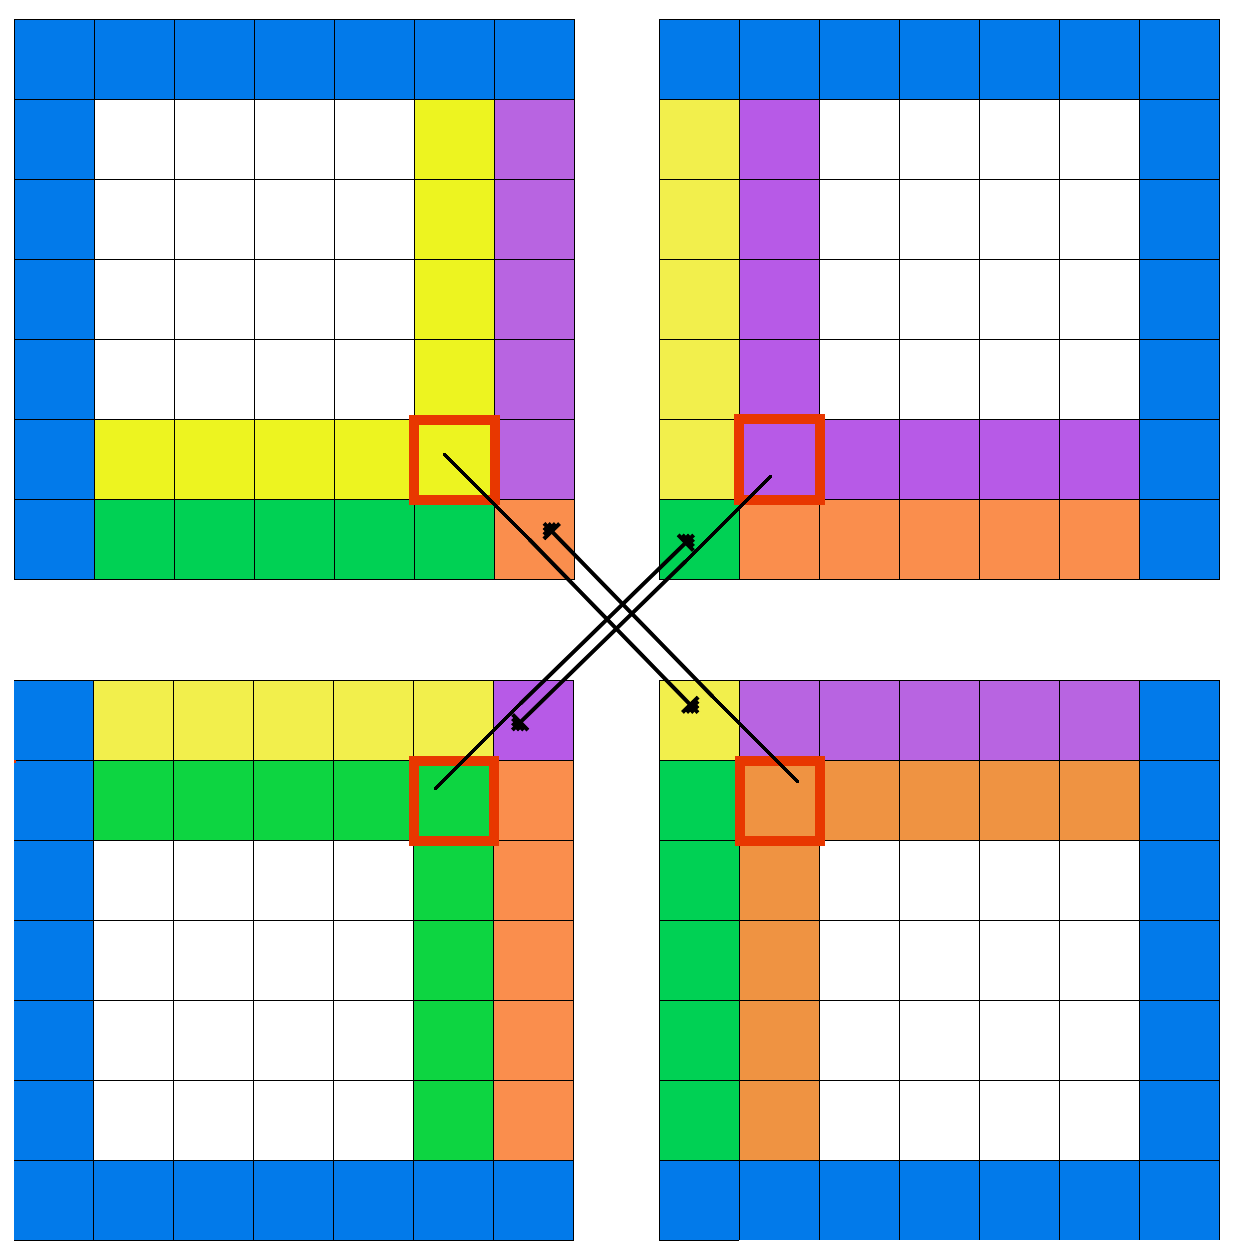
\includegraphics[scale=0.12]{figures/comm3.png}
    \caption{\label{fig:comm_diag}Echanges des coins}
  \end{subfigure}
  \caption{\label{fig:comm_neighbors}Echanges des zones de recouvrement avec MPI\_Neighbor\_alltoallv}
\end{figure}

%\begin{figure}[ht]
%  \centering
%  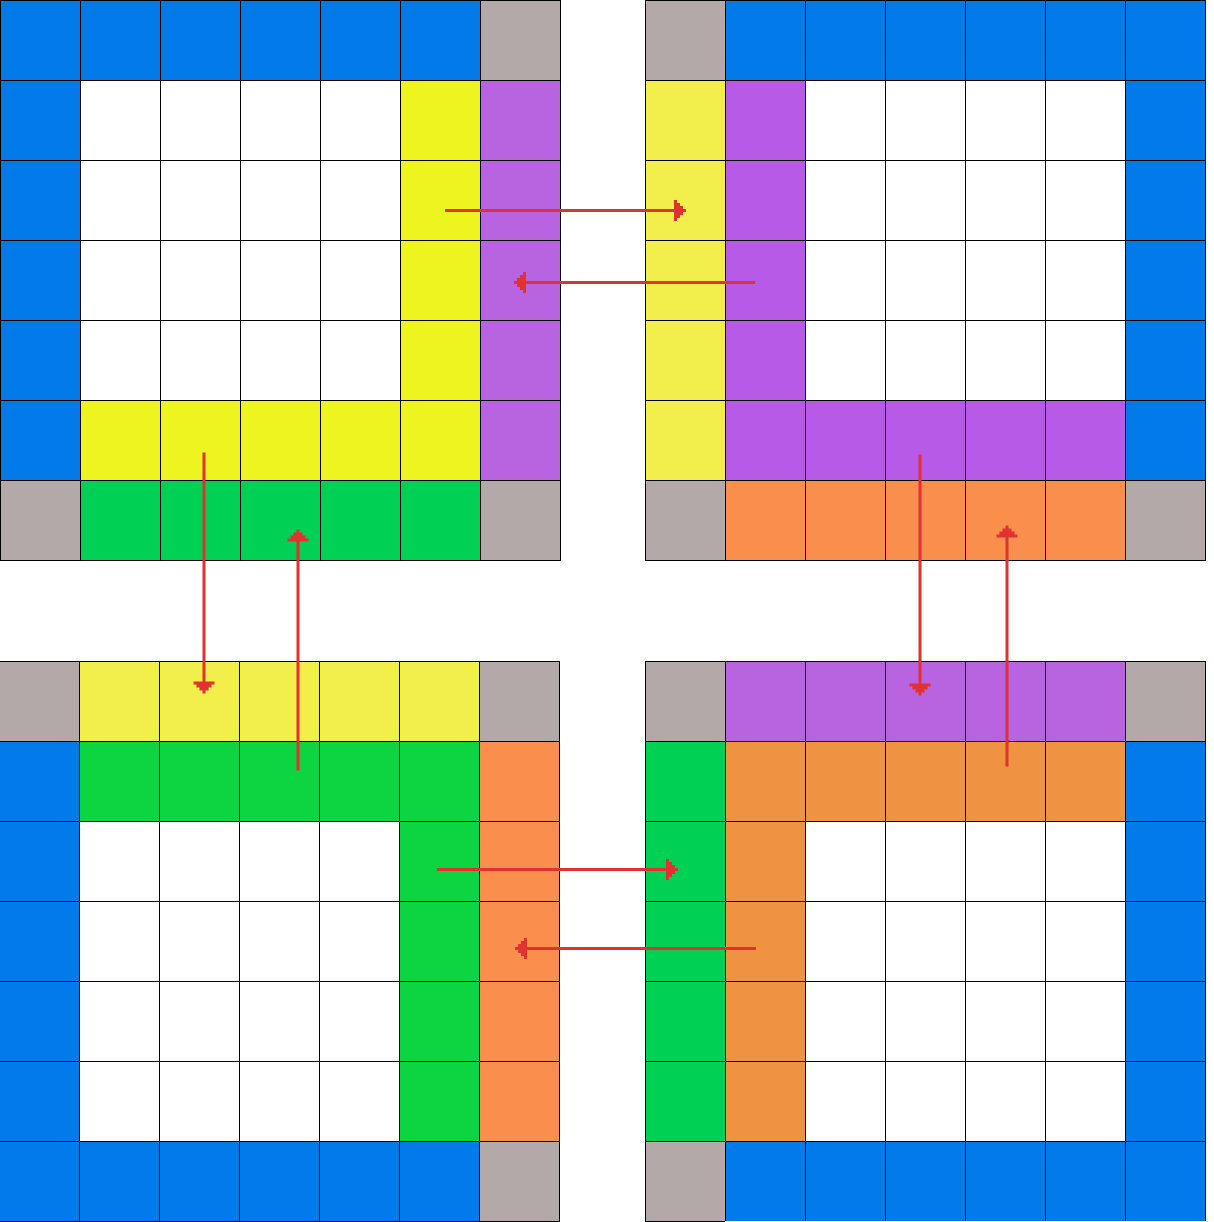
\includegraphics[scale=0.12]{figures/domain-overlap-comms.png}
%  \caption{\label{fig:comm} }
%\end{figure}



\paragraph{}Cependant, comme on peut le voir sur la figure \ref{fig:comm_neigh}, cette fonction ne permet pas d'échanger les coins restés en gris. Il est donc possible d'ajouter des communications en diagonale (fig. \ref{fig:comm_diag}) qui permettront le transfert de ces coins.

\paragraph{}Il est également possible de réaliser les communications illustrées par la figure \ref{fig:comm_synch}. Les communications non-bloquantes se réalisent ici sur une seule dimension à la fois et permettent d'échanger les coins plus facilement. L'avantage de cette seconde option est qu'elle simplifie grandement le code par rapport aux communications en diagonales en réduisant également le nombre de communications. C'est donc cette seconde méthode qui a été utilisée dans NTMIX.

\begin{figure}[!ht]
  \centering
  \begin{subfigure}[b]{0.5\textwidth}
    \centering
    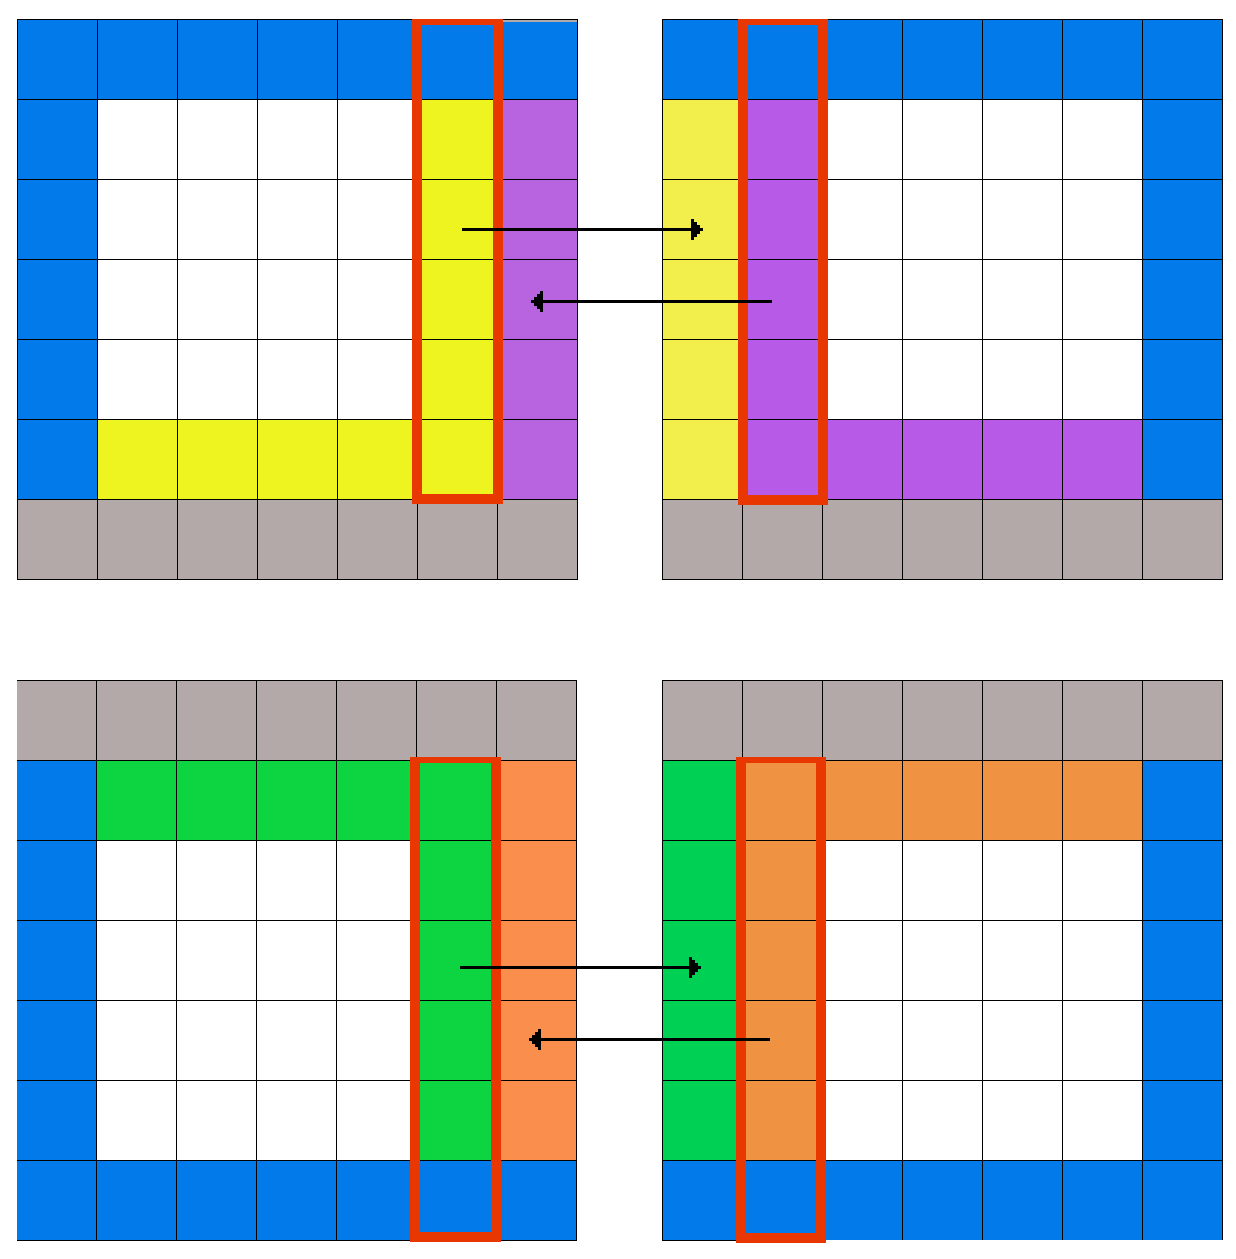
\includegraphics[scale=0.12]{figures/comm1.png}
    \caption{\label{fig:comm1}Echanges sur la dimension $x$}
  \end{subfigure}%
  ~
  \begin{subfigure}[b]{0.5\textwidth}
    \centering
    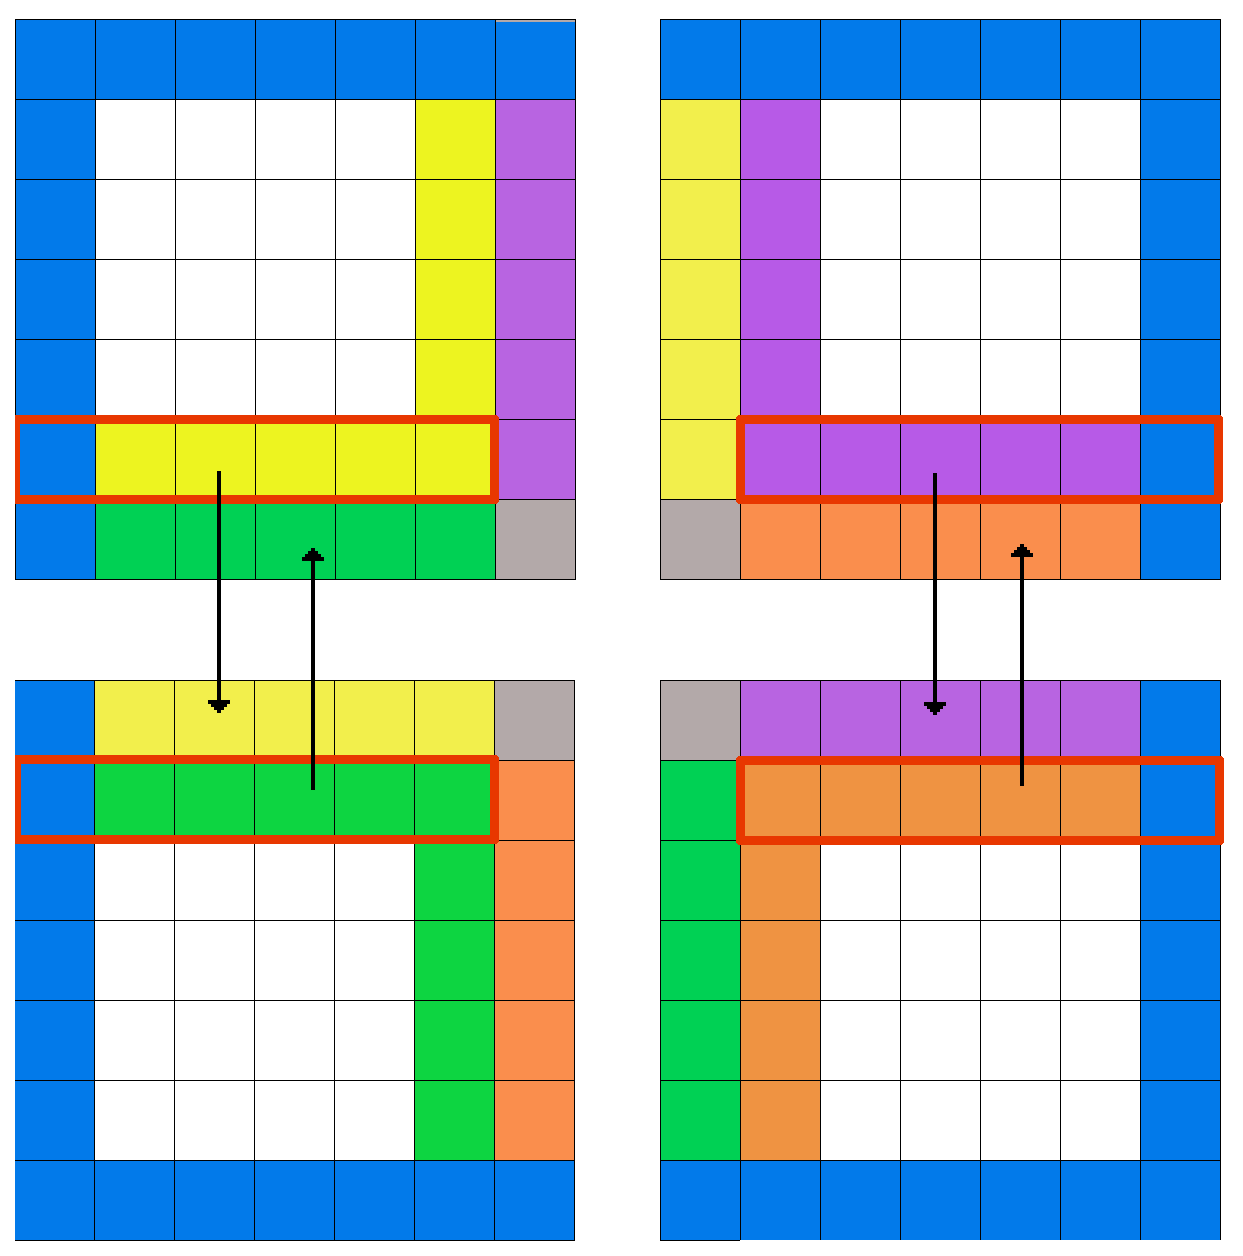
\includegraphics[scale=0.12]{figures/comm2.png}
    \caption{\label{fig:comm2}Echanges sur la dimension $y$}
  \end{subfigure}
  \caption{\label{fig:comm_synch}Echange des zones de recouvrement avec des communications non-bloquantes}
\end{figure}


%\paragraph{}Cependant cette fonction est relativement récente \cite{mpi-3.0} [21 septembre 2012] et peut ne pas être disponible dans les implémentation de MPI présentes sur certains calculateurs qui seront utilisés. Il m'a donc été demandé d'implémenter une seconde méthode dans un soucis de portabilité. C'est une implémentation triviale de la fonction MPI\_Neighbor\_alltoallv (algo. \ref{algo:update}); on parcourt les dimensions du domaine, et pour chaque dimension, on effectue 2 envois et 2 réceptions dans la direction correspondant à cette dimension.



%\begin{algorithm}
%  \caption{update}
%  \label{algo:update}
%  \begin{algorithmic}
%    \STATE {i=1}
%    \FOR{dim=1 \TO dim==ndim } 
%    \STATE {getNeighbors(dim,N1,N2)}
%    \STATE {send(sbuf(offset(i)), N1)}
%    \STATE {recv(rbuf(offset(i)), N1)}
%    \STATE {i=i+1}
%    \STATE {send(sbuf(offset(i)), N2)}
%    \STATE {recv(rbuf(offset(i)), N2)}
%    \ENDFOR
%  \end{algorithmic}
%\end{algorithm}




\subsection{Équilibrage de charge}\label{sec:equilibrage}
Lors d'un tel découpage de domaine, il est nécessaire de s'assurer que la quantité de travail réalisée par chaque processus est semblable à celle des autres. Le but est donc de distribuer le même nombre de mailles sur chaque processus. Dans le cas d'un domaine périodique ce problème n'apparaît pas car chaque processus possède des régions de recouvrement dans toutes les directions (sec. \ref{sec:overlapping}). Cependant, si le domaine possède des frontières physiques, certains sous-domaines n'auront pas la même quantité de points de recouvrement.

\paragraph{}Prenons l'exemple d'un domaine de $100\times100\times100$ points répartis sur une grille de $4\times4\times4$ processus avec un recouvrement de 4: si on découpe le domaine de manière triviale, on obtient donc 64 sous-domaines de taille $25\times25\times25$. Si on ajoute ensuite les points de recouvrement, on retrouve 4 classes de sous-domaines ayant des tailles différentes (fig. \ref{fig:classes}); les coins du domaine auront donc $29\times29\times29$ points (classe C), les autres sous-domaines situés sur les bordures physique auront $33\times29\times29$ points (classe B), les sous-domaines situés sur les faces externes $33\times33\times29$ (classe O) et tous les autres $33\times33\times33$ (classe I: représentée uniquement sur la figure \ref{fig:int-classes}; lorsque le nombre de processus est élevé, cette classe est la plus représentée). Comme on peut le constater dans le tableau \ref{arr:overlap_res}, la charge de calcul est déséquilibrée entre les processus et certain processus (ceux ayant le moins de travail) devront attendre les autres pour les synchronisations présentées en début de partie. Même si ce comportement est moins marqué lorsque les sous-domaines sont plus grands (tab. \ref{arr:overlap_res_big}), il est préférable de l'éviter.
  
Si on ajoute la taille totale du recouvrement avant de découper le domaine, les tailles des domaines internes varient selon les processus mais la taille globale (domaine interne + recouvrement) est identique. Toujours avec l'exemple précédent, si on ajoute la taille de recouvrement à la taille globale, on obtient un domaine global de $124\times124\times124$ points (sur une dimension, les 2 processus se situant aux extrémités possédent 1 seule zone de recouvrement tandis que les 2 autres ont eux 2 régions $(2+2+1+1)\times4=24$) . On divise ensuite ce domaine entre les processus et on obtient cette fois-ci une seule classe de sous-domaine de $31\times31\times31$ points. On joue ici sur la taille du domaine interne pour équilibrer la charge. Un sous-domaine se trouvant sur un coin aura un domaine interne de $27\times27\times27$ alors qu'un sous-domaine de classe A aura $23\times23\times23$ points sur son domaine interne.

Cependant, ces découpages ne prennent pas en compte les communications réalisées entre les différents sous-domaines. Comme il est difficile de prévoir l'importance du coût des communications face au coût des calculs, ces 2 méthodes seront étudiées dans la partie suivante, afin d'essayer de déterminer laquelle convient le mieux lors d'une utilisation réelle de l'application.


\begin{figure}[!ht]
  \centering
  \begin{subfigure}[b]{0.5\textwidth}
    \centering
    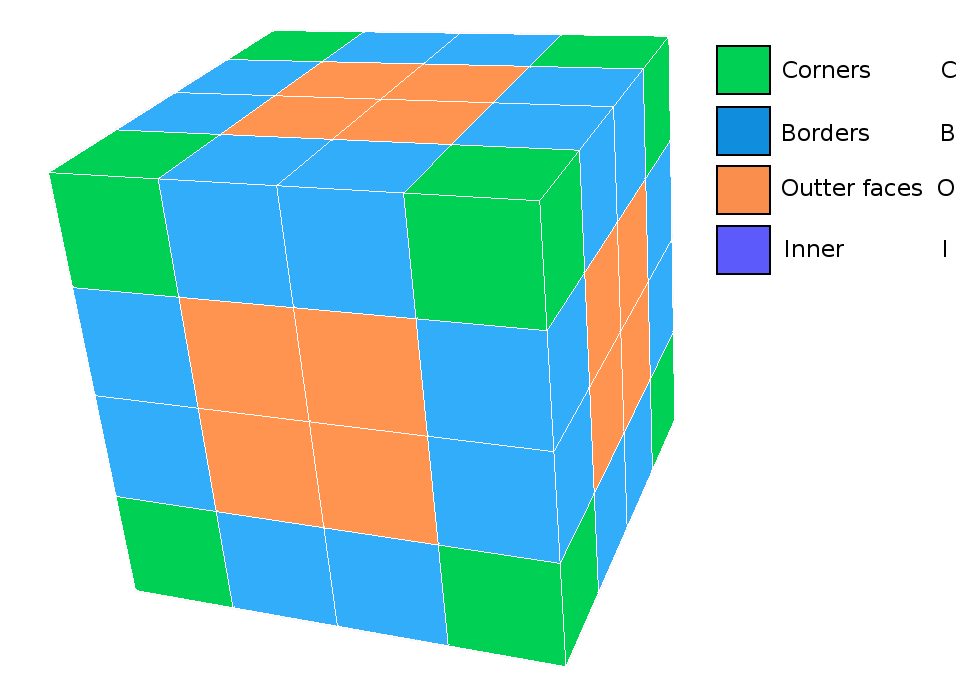
\includegraphics[scale=0.25]{figures/ext-classes.png}
    \caption{\label{fig:ext-classes}Classes externes}
  \end{subfigure}%
  ~
  \begin{subfigure}[b]{0.5\textwidth}
    \centering
    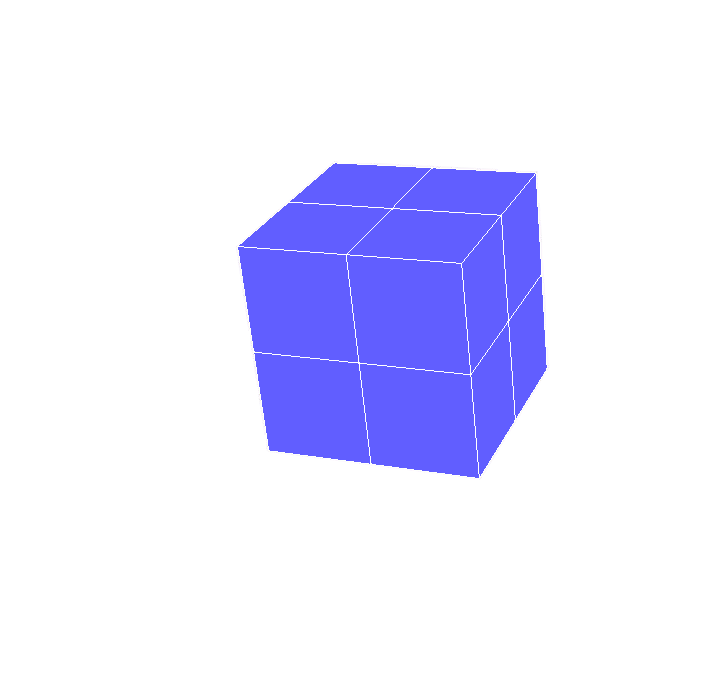
\includegraphics[scale=0.25]{figures/int-classes.png}
    \caption{\label{fig:int-classes}Classes internes}
  \end{subfigure}
  \caption{\label{fig:classes}Classes de sous-domaines}
\end{figure}



\begin{table}[!ht]
  \begin{center}
    \begin{tabular}{|P{2cm}|P{3.5cm}|P{3.5cm}|}
      \hline
      & Taille & Overhead \\ \hline
      C & $29\times29\times29$ & 0\%  \\ \hline
      B & $33\times29\times29$ & 13.8\%  \\ \hline
      O & $33\times33\times29$ & 29.5\%  \\ \hline
      I & $33\times33\times33$ & 47.3\%  \\ \hline      
    \end{tabular}
    \caption{\label{arr:overlap_res}Surcout de calcul - $100\times100\times100$, 64 processus, overlapping 4}
  \end{center}
\end{table}


\begin{table}[!ht]
  \begin{center}
    \begin{tabular}{|P{2cm}|P{3.5cm}|P{3.5cm}|}
      \hline
      & Taille & Overhead \\ \hline
      C & $205\times205\times205$ & 0\%    \\ \hline
      B & $210\times205\times205$ & 2.4\%  \\ \hline
      O & $210\times210\times205$ & 4.9\%  \\ \hline
      I & $210\times210\times210$ & 7.5\%  \\ \hline      
    \end{tabular}
    \caption{\label{arr:overlap_res_big}Surcout de calcul - $1000\times1000\times1000$, 125 processus, overlapping 5}
  \end{center}
\end{table}


\paragraph{}Un déséquilibre de charge peut également apparaître lors de la phase d'initialisation, même si son impact peut être faible face à l'ensemble de la simulation, il est préférable de l'éviter. En effet, il faut éviter qu'un seul processus doive initialiser l'ensemble du domaine puis envoyer les informations calculées à tous les autres processus. Dans le cas de ce programme l'initialisation peut-être réalisée de manière indépendante (sans aucune synchronisation). En effet, les initialisations simples (valeur d'une variable fournie dans le fichier de configuration) ne nécessitent aucun calcul. Les initialisations nécessitant des calculs sont en général fonction de la position d'un point dans le domaine et nécessite un transfert des zones de recouvrement afin de propager les bonnes valeurs avant de démarrer les calculs.


\subsection{Validation}

\paragraph{Cas d'un unique processus}Avant de tester la validité du programme avec plusieurs processus, il est nécessaire de s'assurer qu'il peut être lancé avec un seul processus et que les résultats fournis sont identiques à la version 3D validée à la section \ref{sec:3D-validation}. Même si ce test paraît trivial, il est important de le faire. Il sera également utile de comparer le temps pris par ce test par rapport au temps de la version 3D séquentielle pour estimer le surcout pouvant être induit par l'utilisation de MPI.

\paragraph{Cas avec décomposition de domaine}
Comme vu dans la section \ref{sec:numerical_dom_decompo} le calcul des gradients est dépendant de l'ensemble du domaine. Pour s'assurer de l'exactitude des résultats obtenus dans cette version MPI, j'ai donc utilisé un overlapping assez grand permettant d'obtenir une précision numérique suffisante. J'ai ensuite calculer les valeurs moyennes des champs de la solution afin de les comparer avec ceux obtenus avec la version séquentielle du programme (\ref{sec:3D-validation}).


 \paragraph{}Afin d'étudier la précision de la version parallèle de NTMIX, plusieurs cas de référence ont été exécutés avec la version séquentielle tridimensionnelle en fixant un pas de temps unique. Les mêmes cas tests ont ensuite été réalisés avec la version parallèle, en gardant ce même pas de temps. Cette méthode permet ensuite de mesurer l'erreur moyenne en fonction du nombre de points de recouvrement à l'aide de la formule:

$$ \sqrt{\sum_{i=1}^{n} \frac{({u_p}_i-{u_{ref}}_i)^2}{({u_{ref}}_i)^2}} $$

avec:
\begin{itemize}
\item ${u_p}_i$ la valeur du champ $u$ au point $i$ pour la version parallèle
\item ${u_{ref}}_i$ la valeur du champ $u$ au point $i$ pour la version séquentielle
\end{itemize}
%\begin{table}[!ht]
%  \begin{center}
%    \begin{tabular}{|c|c|c||c|c|c|c||c|c|c|}
%      \hline
%      Overlap & 12 & 11 \\
%      \hline
%      Mean error & 10E-14 & 10E-10 \\
%      \hline
%    
%    \end{tabular}
%    \caption{\label{arr:valid_overlap} Résultats obtenus}
%  \end{center}
%\end{table}
